\section{Figures}\label{sec:2x2sys}
Here is an example of how to include figures and refer to them.
\begin{figure}[ht!]
\floatbox[{\capbeside\thisfloatsetup{capbesideposition={right,center},capbesidewidth=6.3cm}}]{figure}[\FBwidth]
{\caption{Oh figure you so nice.}\label{fig:2x2sys}}
{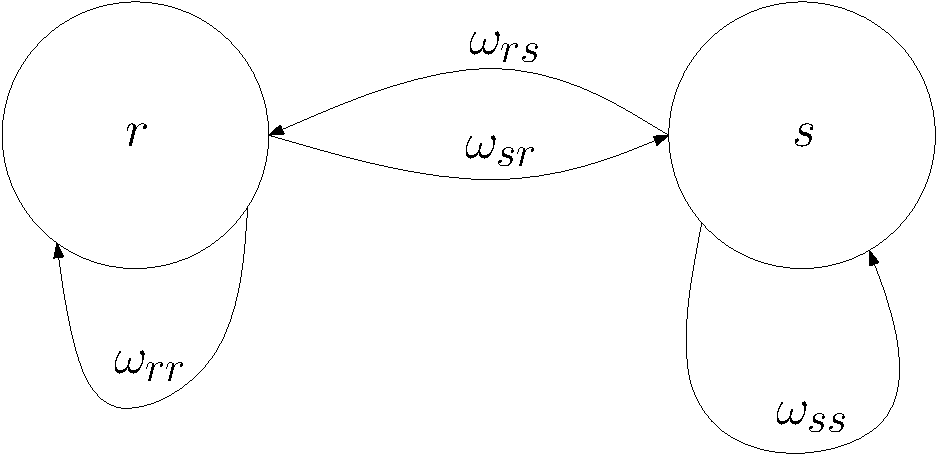
\includegraphics[scale=0.4]{../Graphics/2x2sys}} %tim = l b r t %,trim= 0 0 0 13mm, clip=true
\end{figure}

If we use floatbarrier the figures cant move. However, you probably want them to.
\FloatBarrier


\begin{figure}[ht!]
\subfloat[\label{fig:Dthell2x2Mayor}]{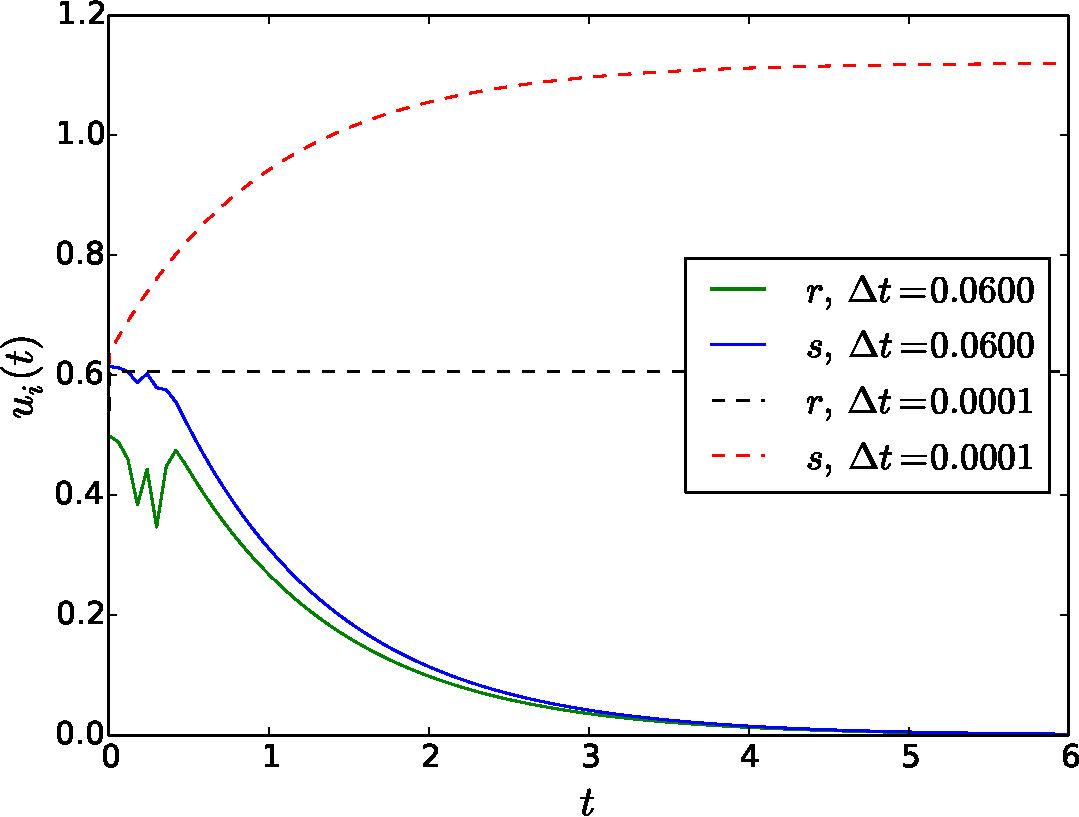
\includegraphics[width=7cm, height=6cm]{../Graphics/Dthell2x2Mayor}}\quad
\subfloat[\label{fig:Dthell2x2MayorCloseup}]{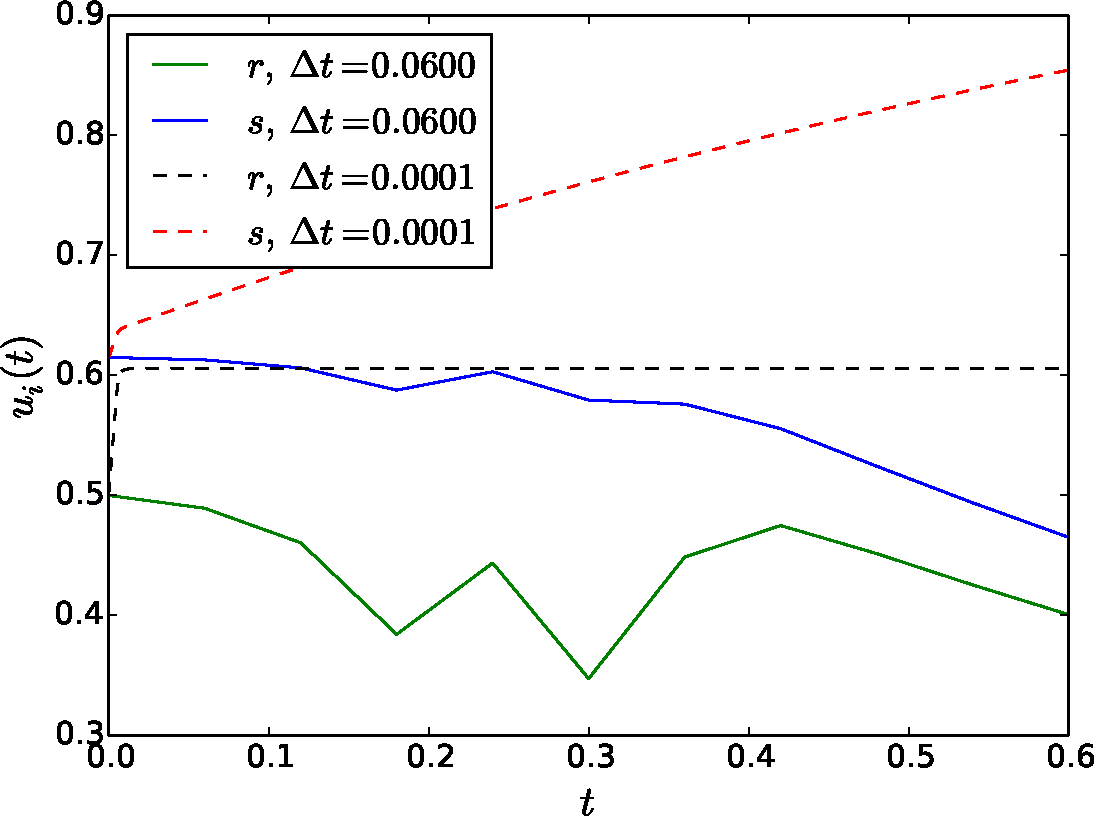
\includegraphics[width=7cm, height=6cm]{../Graphics/Dthell2x2MayorCloseup}}\\
\subfloat[\label{fig:Dthell2x2MayorPhase}]{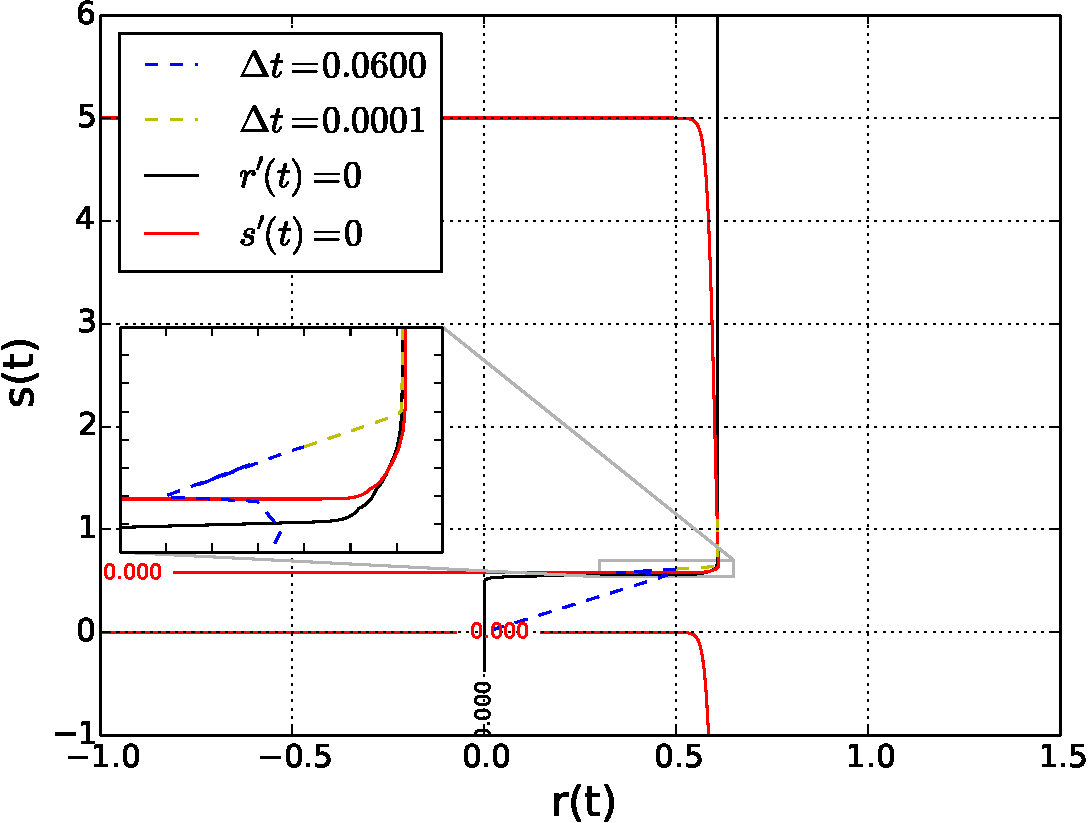
\includegraphics[width=7cm, height=6cm]{../Graphics/Dthell2x2MayorPhase}}\quad
\subfloat[\label{fig:Dthell2x2Spurious}]{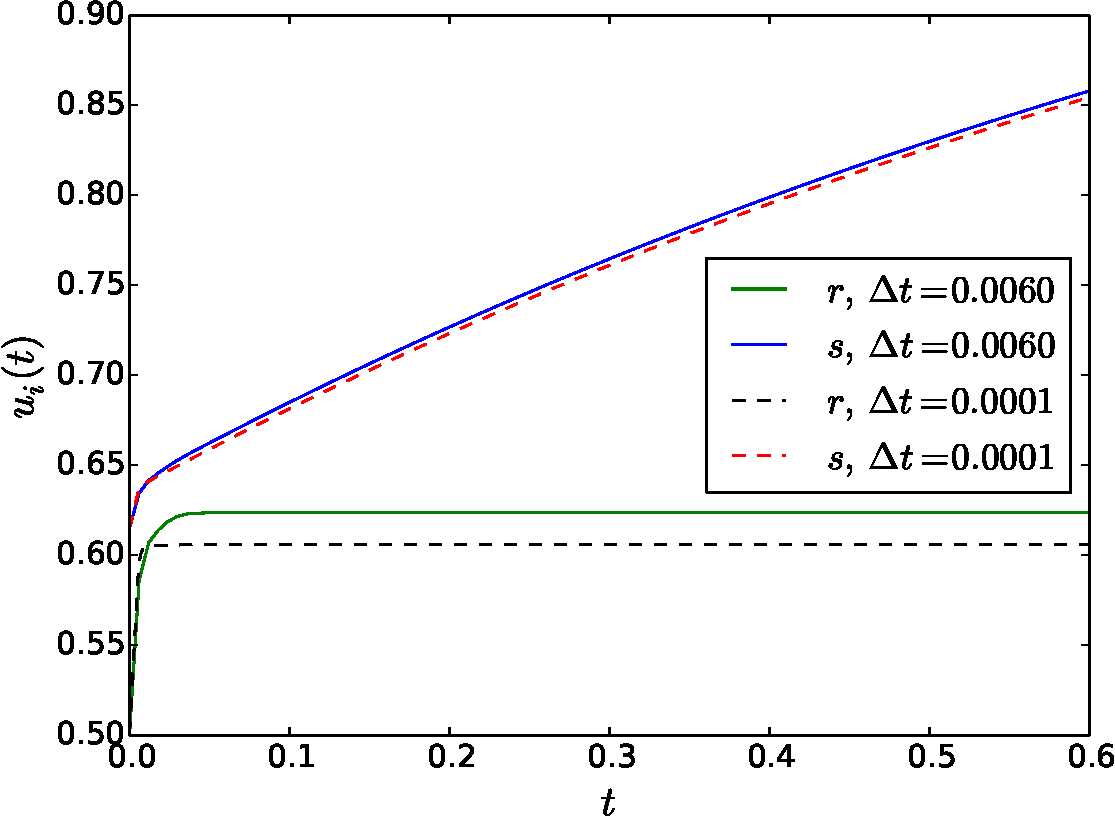
\includegraphics[width=7cm, height=6cm]{../Graphics/Dthell2x2Spurious}}
\caption{I refer to this subfigure \protect\subref{fig:Dthell2x2Spurious}. \label{fig:Dthell2x2WoW}}
\end{figure}
And I want to refer to all of the figures; see \cref{fig:Dthell2x2WoW}. Cleverref is NICE!!

\todo{By the way if you want to add some examples of your own put them in this repo and we can make a collection of \LaTeX howto's}


